\documentclass[compress,aspectratio=169]{beamer}
\usepackage{irbookslide}
\usepackage{irilmenau2}
\usepackage{tikz}
\usepackage{url}
\usepackage{ifxetex}
%\RequireXeTeX
\usepackage{fontspec} % zahteva paket euenc
\usepackage{xunicode}
\usepackage{xltxtra}
\usepackage{polyglossia}
\usepackage{minted}
\usepackage[noend]{algorithmic}
\renewcommand{\algorithmicrequire}{\textbf{Input:}}
\renewcommand{\algorithmicensure}{\textbf{Output:}}
\renewcommand{\algorithmiccomment}[1]{\hfill \{\myred{#1}\}}
\usepackage{xcolor,colortbl}
\usepackage{textcomp}
\usepackage{unicode-math}
%\setdefaultlanguage[script=Latin]{serbian}

\title{Red sa prioritetom, heap, adaptivni RSP}
\author{\textcopyright \ \ Goodrich, Tamassia, Goldwasser}
\institute{Katedra za informatiku, Fakultet tehničkih nauka, Univerzitet u
Novom Sadu}
\date{2021.}
\subject{Predavanja sa ASP}

\begin{document}

\frame{\titlepage}

\section[Red sa prioritetom]{Red sa prioritetom}
\begin{frame}[fragile]
  \frametitle{Red sa prioritetom}
  \begin{itemize}
    \item \myred{red sa prioritetom} čuva kolekciju elemenata 
    \item svaki element je par (\myred{ključ}, \myred{vrednost})
    \item osnovne operacije:
    \begin{itemize}
      \item \myred{add}($k, x$): dodaje element sa ključem $k$ i vrednošču $x$
      \item \myred{remove\_min}(): uklanja element sa najmanjim ključem 
    \end{itemize}
    \item dodatne operacije:
    \begin{itemize}
      \item \myred{min}(): vraća, ali ne uklanja, element sa najmanjim ključem
      \item \myred{len}(), \myred{is\_empty}() 
    \end{itemize}
  \end{itemize}
\end{frame}

\begin{frame}[fragile,shrink=10]
  \frametitle{Primer operacija nad redom sa prioritetom}
\begin{center}
\begin{tabular}{lcl}
\textbf{operacija} & \textbf{rezultat} & \textbf{sadržaj reda} \\
\hline \hline
\texttt{P.add(5, A)} & -- & [(5,A)] \\ 
\texttt{P.add(9, C)} & -- & [(5,A), (9,C)] \\ 
\texttt{P.add(3, B)} & -- & [(3,B), (5,A), (9,C)] \\ 
\texttt{P.add(7, D)} & -- & [(3,B), (5,A), (7,D), (9,C)] \\ 
\texttt{P.min()} & (3,B) & [(3,B), (5,A), (7,D), (9,C)] \\ 
\texttt{P.remove\_min()} & (3,B) & [(5,A), (7,D), (9,C)] \\ 
\texttt{P.remove\_min()} & (5,A) & [(7,D), (9,C)] \\ 
\texttt{len(P)} & 2 & [(7,D), (9,C)] \\
\texttt{P.remove\_min()} & (7,D) & [(9,C)] \\ 
\texttt{P.remove\_min()} & (9,C) & [ ] \\ 
\texttt{P.is\_empty()} & True & [ ] \\ 
\texttt{P.remove\_min()} & greška & [ ]
\end{tabular}
\end{center}
\end{frame}

\begin{frame}[fragile]
  \frametitle{Ključevi i relacija poretka}
  \begin{itemize}
    \item ključevi mogu biti bilo kog tipa za koga je definisana relacija poretka
    \item elementi u redu mogu imati jednake ključeve -- u tom slučaju se primenjuje FIFO princip
    \item relacija poretka
    \begin{itemize}
      \item refleksivna: $x\leq x$
      \item antisimetrična: $x\leq y \land y\leq x \, \Rightarrow \, x = y$
      \item tranzitivna: $x\leq y \land y\leq z \, \Rightarrow \, x\leq z$
    \end{itemize}
  \end{itemize}
\end{frame}

\begin{frame}[fragile,shrink]
  \frametitle{Element RSP}
\begin{minted}[linenos=false]{python}
class PriorityQueueItem:
  def __init__(self, k, v):
    self.key = k
    self.value = v
    
  def __lt__(self, other):
    return self.key < other.key
    
  def __le__(self, other):
    return self.key <= other.key
\end{minted}
\end{frame}

\begin{frame}[fragile]
\frametitle{Implementacija RSP}
\begin{columns}
  \begin{column}[c]{5.5cm}
    \begin{itemize}
      \item implementacija sa \textbf{nesortiranom} listom
      \item \myred{add} je $O(1)$ jer dodavanje možemo raditi na bilo kom kraju liste
      \item \myred{remove\_min} i \myred{min} su $O(n)$ jer moramo tražiti najmanji ključ u listi
    \end{itemize}
    \begin{center}
      
\includegraphics[width=5cm]{asp-09-pic01a.png}
    \end{center}
  \end{column}
  \begin{column}[c]{5.5cm}
    \begin{itemize}
      \item implementacija sa \textbf{sortiranom} listom
      \item \myred{add} je $O(n)$ jer moramo da nađemo pravo mesto za ubacivanje novog elementa
      \item \myred{remove\_min} i \myred{min} su $O(1)$ jer je najmanji ključ uvek na početku
    \end{itemize}
    \begin{center}
      
\includegraphics[width=5cm]{asp-09-pic01b.png}
    \end{center}
  \end{column}
\end{columns}
\end{frame}

\begin{frame}[fragile,shrink]
  \frametitle{RSP sa nesortiranom listom}
\begin{minted}[linenos=false]{python}
class UnsortedPriorityQueue:
  def __init__(self):
    self._data = SingleList()
    
  def add(self, key, value):
    newest = PriorityQueueItem(key, value) 
    self._data.add_last(newest)
    
  def _find_min(self)
    if self.is_empty():
      raise Empty('Queue is empty')
    smallest = self._data.first()
    current = smallest.next
    while current is not None:
      if current.element < smallest.element:
        smallest = curr
      current = current.next
    return smallest
  
  def remove_min(self):
    p = self._find_min()
    item = self._data.delete(p)
    return (item.key, item.value)
\end{minted}
\end{frame}

\begin{frame}[fragile,shrink]
  \frametitle{RSP sa sortiranom listom}
\begin{minted}[linenos=false]{python}
class SortedPriorityQueue:
  def __init__(self):
    self._data = SingleList()
    
  def add(self, key, value):
    newest = PriorityQueueItem(key, value)
    current = self._data.first()
    while current is not None and newest < current.element:
      current = current.next 
    if current is None:
      self._data.add_first(newest)
    else:
      self._data.add_after(current, newest)
    
  def remove_min(self):
    if self.is_empty():
      raise Empty('Queue is empty')
    item = self._data.delete(self._data.first())
    return (item.key, item.value)
\end{minted}
\end{frame}

\section[Heap]{Heap}
\begin{frame}[fragile]
  \frametitle{Heap}
  \begin{itemize}
    \item \myred{heap} je binarno stablo\ldots 
    \item \ldots čiji elementi su uređeni parovi (\myred{ključ}, \myred{vrednost})
    \item \ldots i koje zadovoljava još 2 uslova:
    \begin{itemize}
      \item \textbf{redosled}: za svaki čvor $n$ osim korena ključ od $n$ je veći ili jednak ključu roditelja od $n$
      \item \textbf{kompletnost}: heap visine $h$ ima nivoe $0, 1, 2,\ldots h-1$ sa maksimalnim brojem čvorova ($i$-ti nivo ima $2^i$ čvorova za $0\leq i\leq
      h-1$)
    \end{itemize}
  \end{itemize}
  \begin{center}
    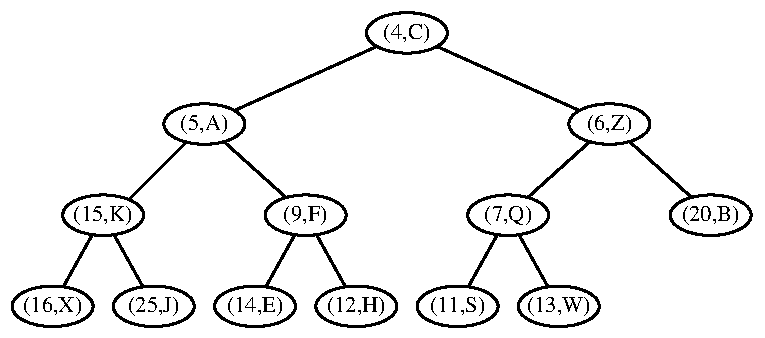
\includegraphics[width=8.5cm]{asp-09-pic02.pdf}
  \end{center}
\end{frame}

\begin{frame}[fragile]
  \frametitle{Heap}
  \begin{itemize}
    \item \myred{poslednji čvor} je poslednji čvor sa \textbf{desne} strane na
    najnižem nivou stabla
  \end{itemize}
  \begin{center}
    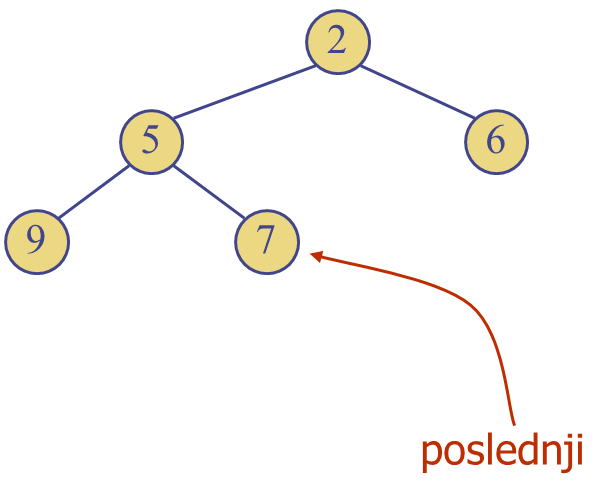
\includegraphics[width=5cm]{asp-09-pic03.png}
  \end{center}
\end{frame}

\begin{frame}[fragile]
  \frametitle{Dubina heapa}
  \begin{itemize}
    \item \textbf{teorema:} heap koji čuva $n$ ključeva ima dubinu $O(\log n)$
    \begin{itemize}
      \item $h$: visina heapa sa $n$ ključeva
      \item ima $2^i$ ključeva na dubini $i = 0, \ldots h-1$ i bar jedan ključ
      na dubini $h$
      \item prema tome, $n \geq 1 + 2 + 4 + \ldots 2^{h-1} + 1$
      \item $n \geq 2^h$
      \item $h \leq \log n$
    \end{itemize}
  \end{itemize}
  \begin{center}
    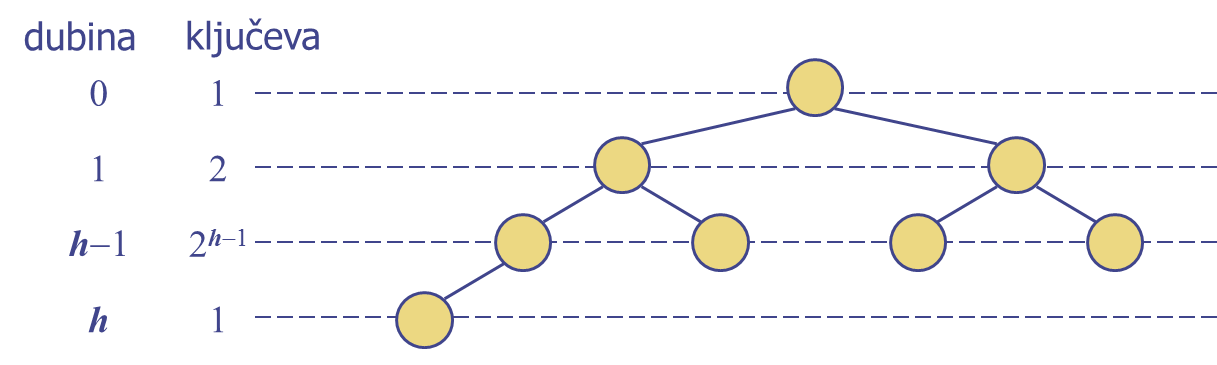
\includegraphics[width=9cm]{asp-09-pic04.png}
  \end{center}
\end{frame}

\begin{frame}[fragile]
  \frametitle{Heap i red sa prioritetom}
  \begin{itemize}
    \item red sa prioritetom možemo implementirati pomoću heapa
    \item u svakom čvoru stabla čuvamo par (ključ, vrednost)
    \item pamtimo položaj poslednjeg čvora
  \end{itemize}
  \begin{center}
    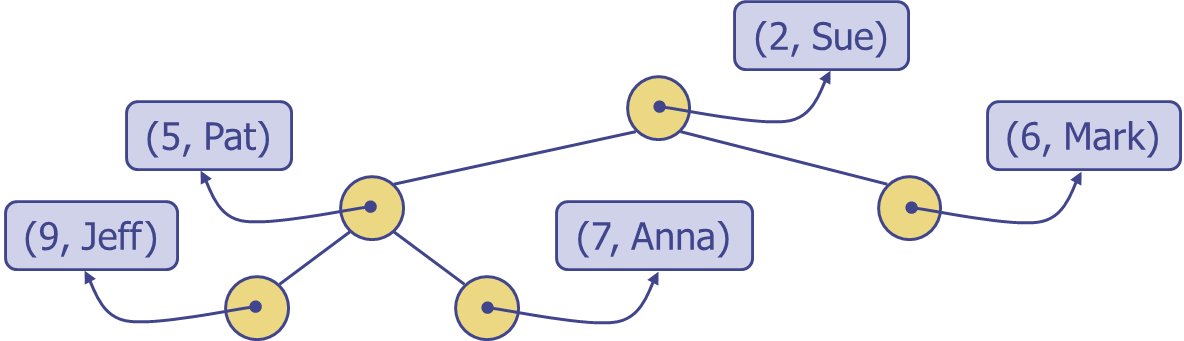
\includegraphics[width=9cm]{asp-09-pic05.png}
  \end{center}
\end{frame}

\begin{frame}[fragile]
  \frametitle{Dodavanje u heap}
  \begin{columns}
    \begin{column}[c]{6cm}
      \begin{itemize}
        \item \myred{add} u redu sa prioritetom se implementira kao dodavanje
        u heap
        \item dodavanje se vrši u tri koraka
        \begin{itemize}
          \item[1] nađi novi poslednji čvor $z$
          \item[2] sačuvaj ($k$, $v$) u $z$
          \item[3] restauriraj pravilan \textbf{redosled}
        \end{itemize}
      \end{itemize}
    \end{column}
    \begin{column}[c]{5cm}
      \begin{center}
        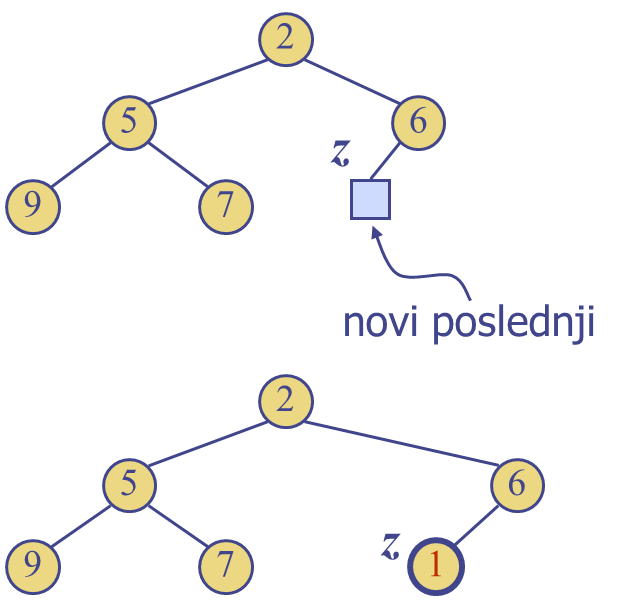
\includegraphics[width=5cm]{asp-09-pic06.png}
      \end{center}
    \end{column}
  \end{columns}
\end{frame}

\begin{frame}[fragile]
  \frametitle{Dodavanje u heap: restauracija redosleda}
  \begin{itemize}
    \item nakon dodavanja novog ključa $k$ redosled čvorova može biti narušen
    \item algoritam \myred{upheap} uspostavlja korektan redosled zamenom $k$ duž
    putanje od novog čvora prema korenu
    \item \textbf{upheap} se završava kada $k$ dođe u koren ili njegov roditelj
    ima ključ manji ili jednak $k$
    \item pošto heap ima visinu $O(\log n)$, upheap radi u $O(\log n)$ vremenu
  \end{itemize}
  \begin{center}
    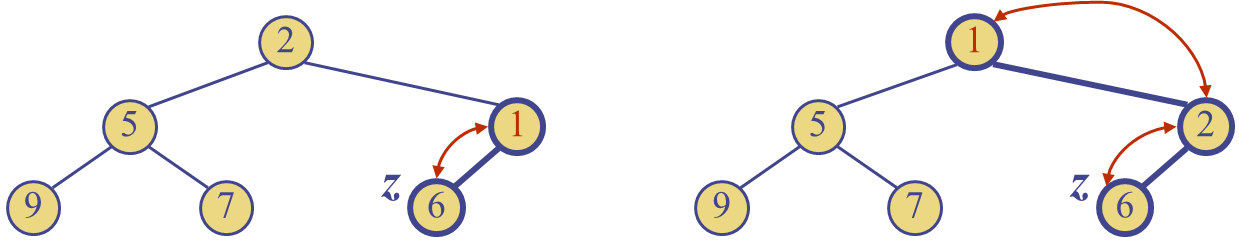
\includegraphics[width=10cm]{asp-09-pic07.png}
  \end{center}
\end{frame}

\begin{frame}[fragile]
  \frametitle{Uklanjanje iz heapa}
  \begin{columns}
    \begin{column}[c]{6cm}
      \begin{itemize}
        \item \myred{remove\_min} se implementira kao uklanjanje korena iz heapa
        \item uklanjanje se vrši u tri koraka
        \begin{itemize}
          \item[1] na mesto korena stavi poslednji čvor $w$
          \item[2] ukloni $w$
          \item[3] restauriraj pravilan \textbf{redosled}
        \end{itemize}
      \end{itemize}
    \end{column}
    \begin{column}[c]{5cm}
      \begin{center}
        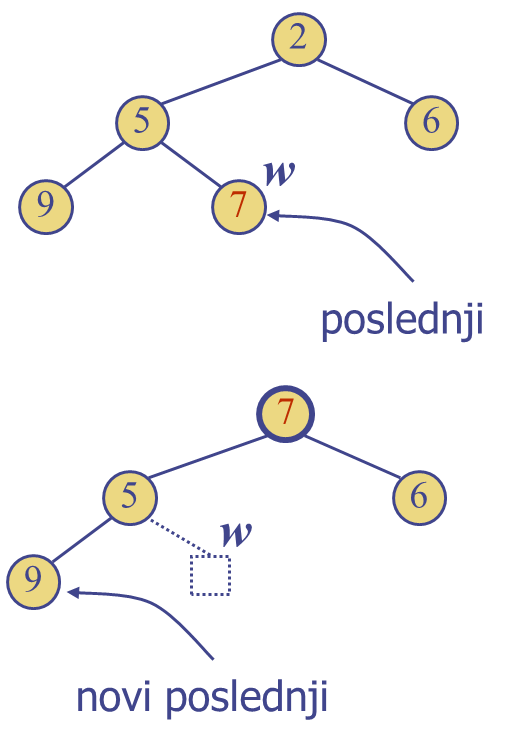
\includegraphics[width=4cm]{asp-09-pic08.png}
      \end{center}
    \end{column}
  \end{columns}
\end{frame}

\begin{frame}[fragile]
  \frametitle{Uklanjanje iz heapa: restauracija redosleda}
  \begin{itemize}
    \item nakon smeštanja ključa $k$ poslednjeg čvora u koren redosled čvorova
    može biti narušen
    \item algoritam \myred{downheap} uspostavlja korektan redosled zamenom $k$
    duž putanje od korena
    \item \textbf{downheap} se završava kada $k$ dođe u list ili njegova
    deca imaju ključeve veće ili jednake $k$
    \item pošto heap ima visinu $O(\log n)$, downheap radi u $O(\log n)$ vremenu
  \end{itemize}
  \begin{center}
    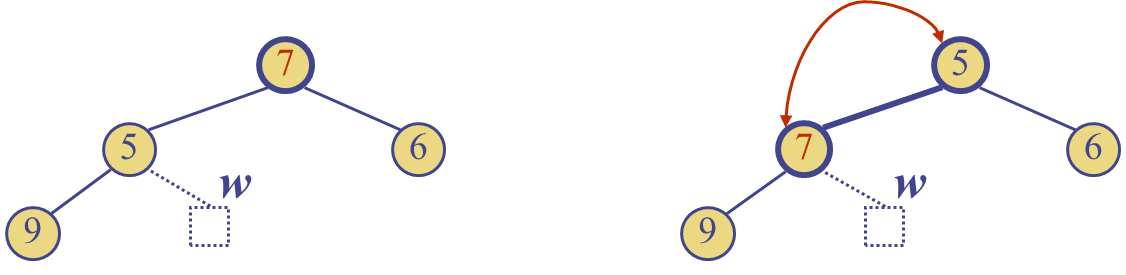
\includegraphics[width=10cm]{asp-09-pic09.png}
  \end{center}
\end{frame}

\begin{frame}[fragile]
  \frametitle{Nađi mesto za novi poslednji prilikom dodavanja}
  \begin{itemize}
    \item mesto za novi poslednji čvor se može naći prolaskom kroz putanju od
    $O(\log n)$ čvorova
    \begin{itemize}
      \item idi prema gore dok ne dođeš do korena ili nečijeg levog deteta
      \item ako si došao do nečijeg levog deteta, idi na desno dete
      \item idi prema dole levo dok ne dođeš do lista
    \end{itemize}
    \item sličan je i algoritam prilikom uklanjanja
  \end{itemize}
  \begin{center}
    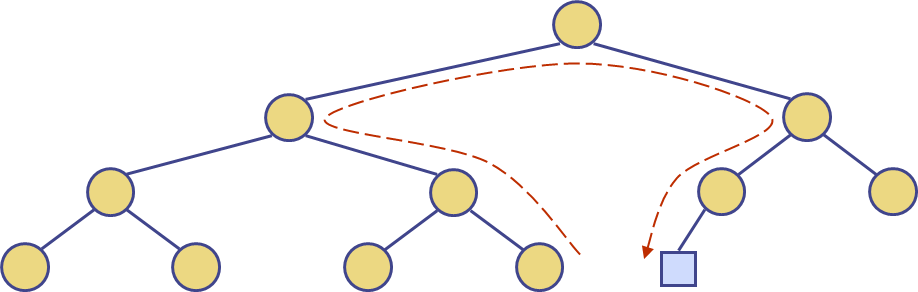
\includegraphics[width=10cm]{asp-09-pic10.png}
  \end{center}
\end{frame}

\begin{frame}[fragile]
  \frametitle{Implementacija heapa pomoću niza}
  \begin{columns}
    \begin{column}[c]{6cm}
      \begin{itemize}
        \item heap sa $n$ ključeva se može smestiti u niz dužine $n$
        \item za čvor ranga $i$
        \begin{itemize}
          \item levo dete ima rang $2i+1$
          \item desno dete ima rang $2i+2$
        \end{itemize}
        \item veze između čvorova se ne čuvaju
        \item dodavanje se svodi na upis čvora ranga $n+1$
        \item uklanjanje se svodi na uklanjanje čvora ranga $n$
      \end{itemize}
    \end{column}
    \begin{column}[c]{5cm}
      \begin{center}
        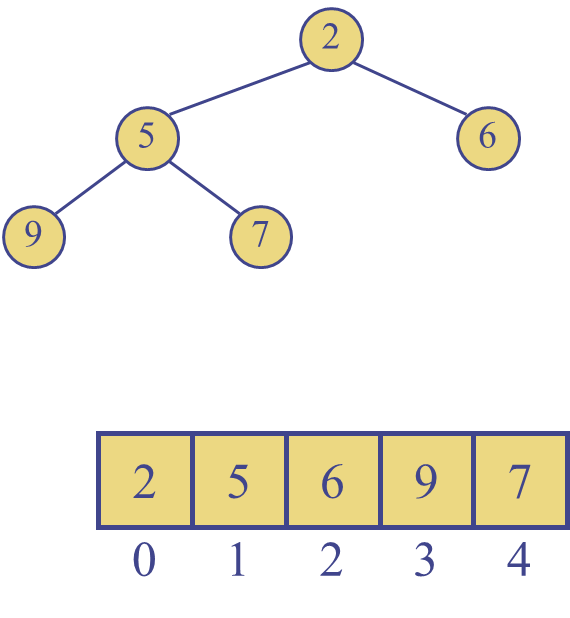
\includegraphics[width=4cm]{asp-09-pic11.png}
      \end{center}
    \end{column}
  \end{columns}
\end{frame}

\begin{frame}[fragile,shrink]
  \frametitle{Heap u Pythonu $_1$}
\begin{minted}[linenos=false]{python}
class HeapPriorityQueue:
  def __init__(self):
    self._data = []
  
  def _parent(self, j):
    return (j-1)//2
    
  def _left(self, j):
    return 2*j+1
  
  def _right(self, j):
    return 2*j+2
    
  def _has_left(self, j):
    return self._left(j) < len(self._data)
    
  def _has_right(self, j):
    return self._right(j) < len(self._data)
    
  def _swap(self, i, j):
    self._data[i], self._data[j] = self._data[j], self._data[i]
\end{minted}
\end{frame}

\begin{frame}[fragile,shrink]
  \frametitle{Heap u Pythonu $_2$}
\begin{minted}[linenos=false]{python}
  def _upheap(self, j):
    parent = self._parent(j)
    if j > 0 and self._data[j] < self._data[parent]:
      self._swap(j, parent)
      self._upheap(parent)
  
  def _downheap(self, j):
    if self._has_left(j):
      left = self._left(j)
      small_child = left
      if self._has_right(j):
        right = self._right(j)
        if self._data[right] < self._data[left]:
          small_child = right
      if self._data[small_child] < self._data[j]:
        self._swap(j, small_child)
        self._downheap(small_child)
\end{minted}
\end{frame}

\begin{frame}[fragile,shrink]
  \frametitle{Heap u Pythonu $_3$}
\begin{minted}[linenos=false]{python}
  def add(self, key, value):
    self._data.append(PriorityQueueItem(key, value))
    self._upheap(len(self._data)-1)
    
  def min(self):
    if self.is_empty():
      raise Empty('Queue is empty')
    item = self._data[0]
    return (item.key, item.value)
    
  def remove_min(self):
    if self.is_empty():
      raise Empty('Queue is empty')
    self._swap(0, len(self._data)-1)
    item = self._data.pop()
    self._downheap(0)
    return (item.key, item.value)  
\end{minted}
\end{frame}

\begin{frame}[fragile]
  \frametitle{Spajanje dva heapa}
  \begin{columns}
    \begin{column}[c]{6cm}
      \begin{itemize}
        \item imamo dva heapa i ključ $k$
        \item kreiramo novi heap sa korenom $k$ i dva heapa kao podstabla
        \item pokrenemo \textbf{downheap} da restauriramo redosled
      \end{itemize}
    \end{column}
    \begin{column}[c]{5cm}
      \begin{center}
        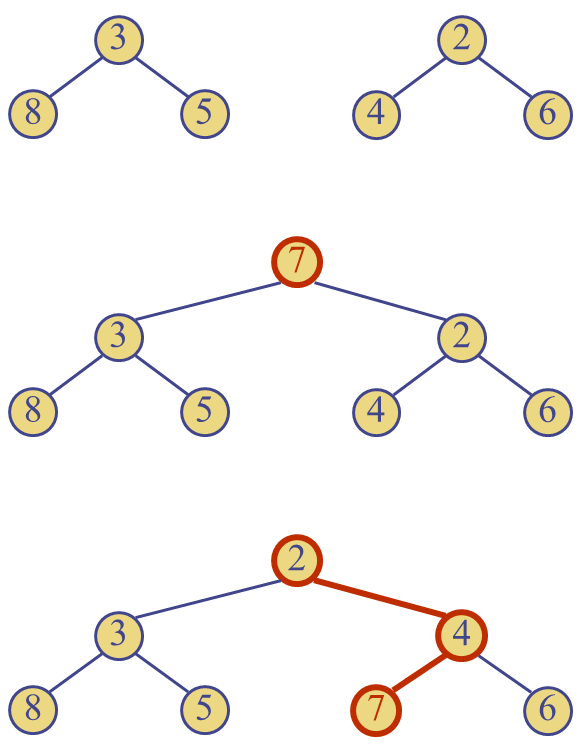
\includegraphics[width=5cm]{asp-09-pic12.png}
      \end{center}
    \end{column}
  \end{columns}
\end{frame}

\begin{frame}[fragile]
  \frametitle{Konstrukcija heapa od dole (bottom-up)}
  \begin{columns}
    \begin{column}[c]{6cm}
      \begin{itemize}
        \item možemo da napravimo heap sa $n$ ključeva pomoću bottom-up
        spajanja u $O(\log n)$ koraka
        \item u $i$-tom koraku, par heapova sa $2^i-1$ ključeva se spajaju u
        heap sa $2^{i+1}-1$ ključeva
        \end{itemize}
    \end{column}
    \begin{column}[c]{5cm}
      \begin{center}
        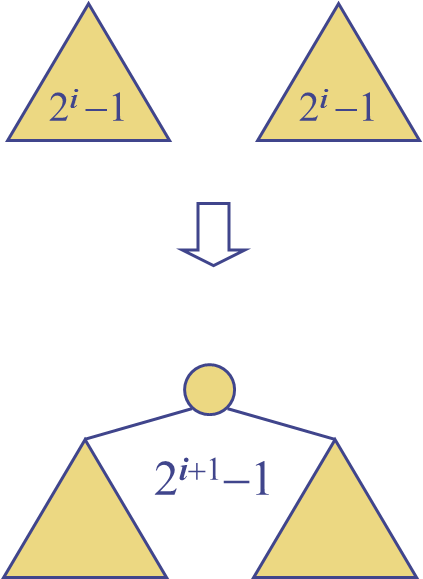
\includegraphics[width=4cm]{asp-09-pic13.png}
      \end{center}
    \end{column}
  \end{columns}
\end{frame}

\begin{frame}[fragile]
  \frametitle{Bottom-up primer $_1$}
  \begin{center}
    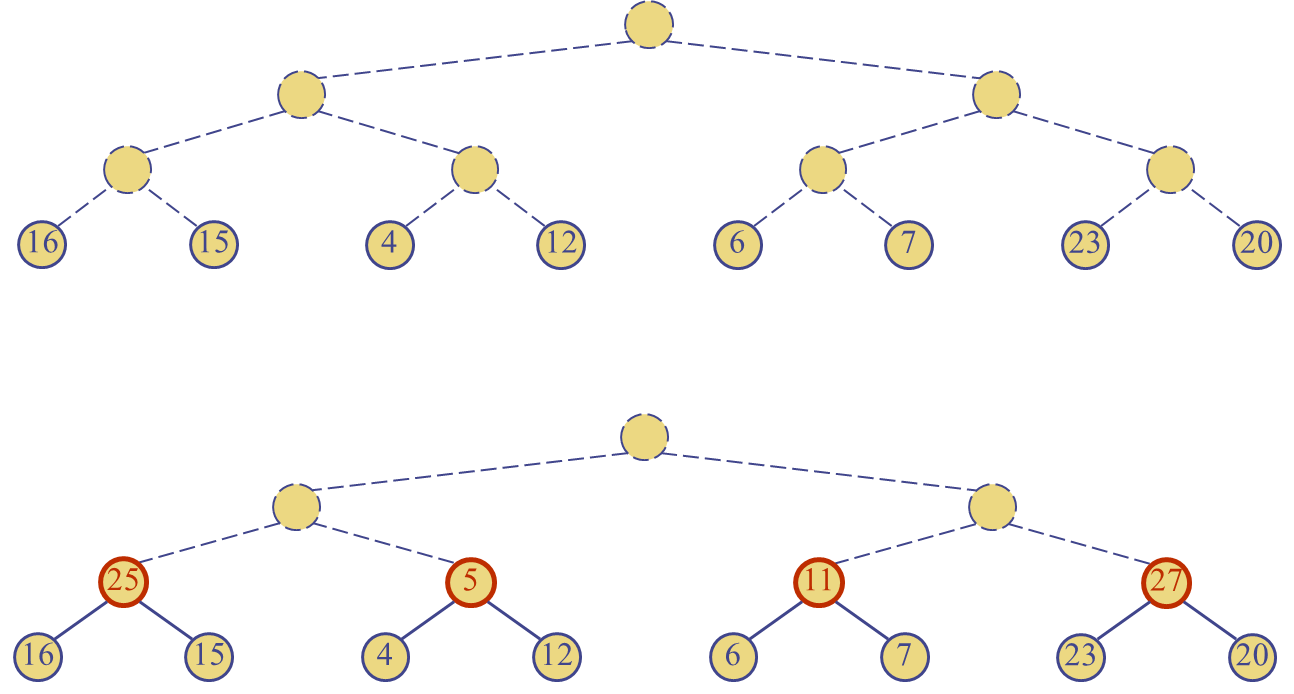
\includegraphics[width=10cm]{asp-09-pic14.png}
  \end{center}
\end{frame}

\begin{frame}[fragile]
  \frametitle{Bottom-up primer $_2$}
  \begin{center}
    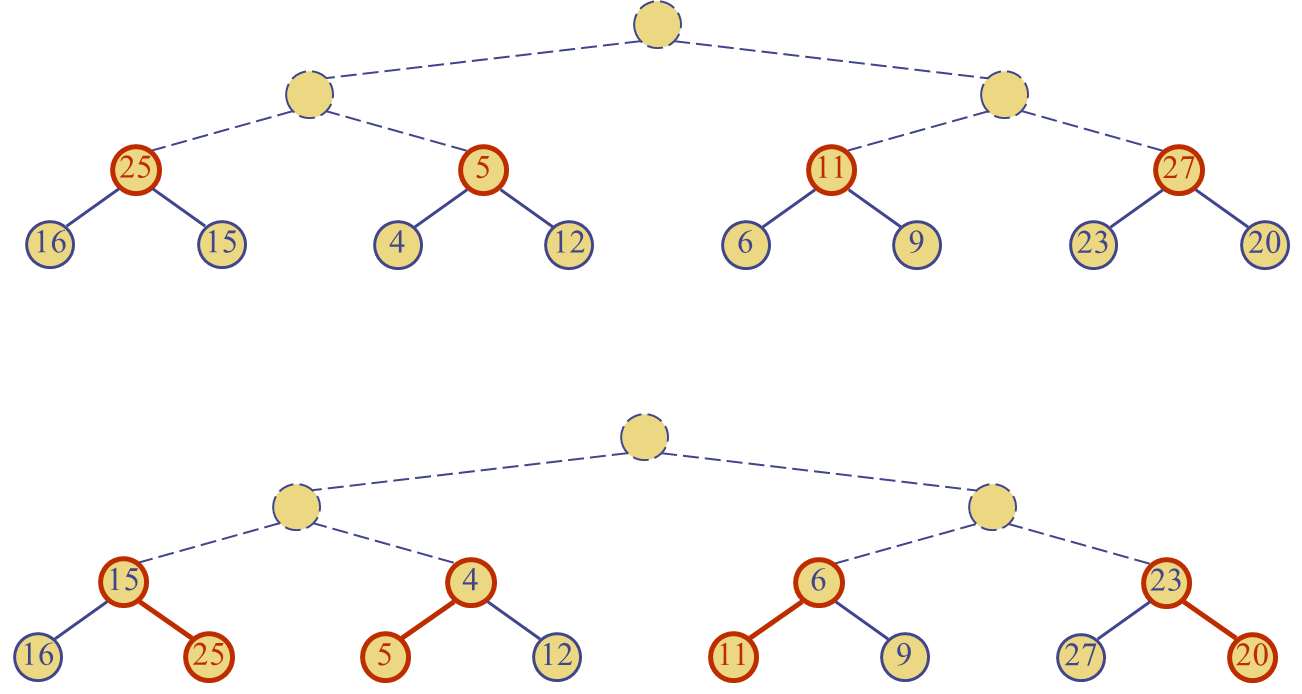
\includegraphics[width=10cm]{asp-09-pic15.png}
  \end{center}
\end{frame}

\begin{frame}[fragile]
  \frametitle{Bottom-up primer $_3$}
  \begin{center}
    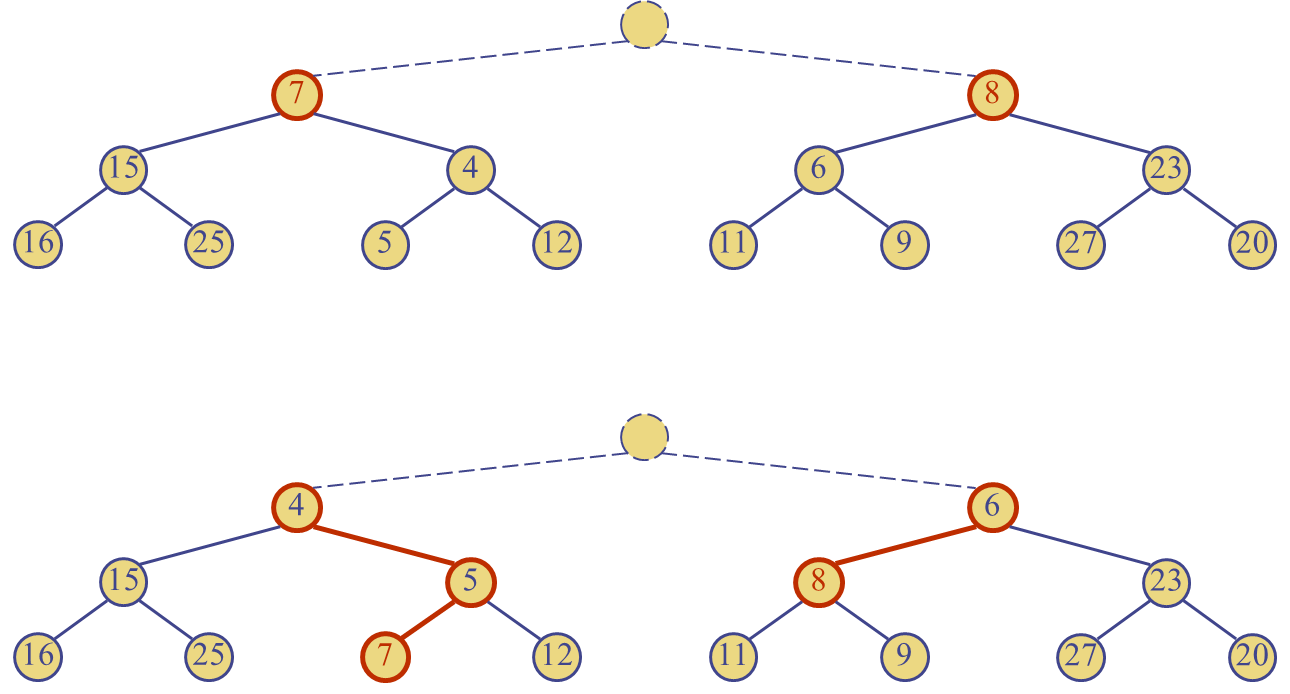
\includegraphics[width=10cm]{asp-09-pic16.png}
  \end{center}
\end{frame}

\begin{frame}[fragile]
  \frametitle{Bottom-up primer $_4$}
  \begin{center}
    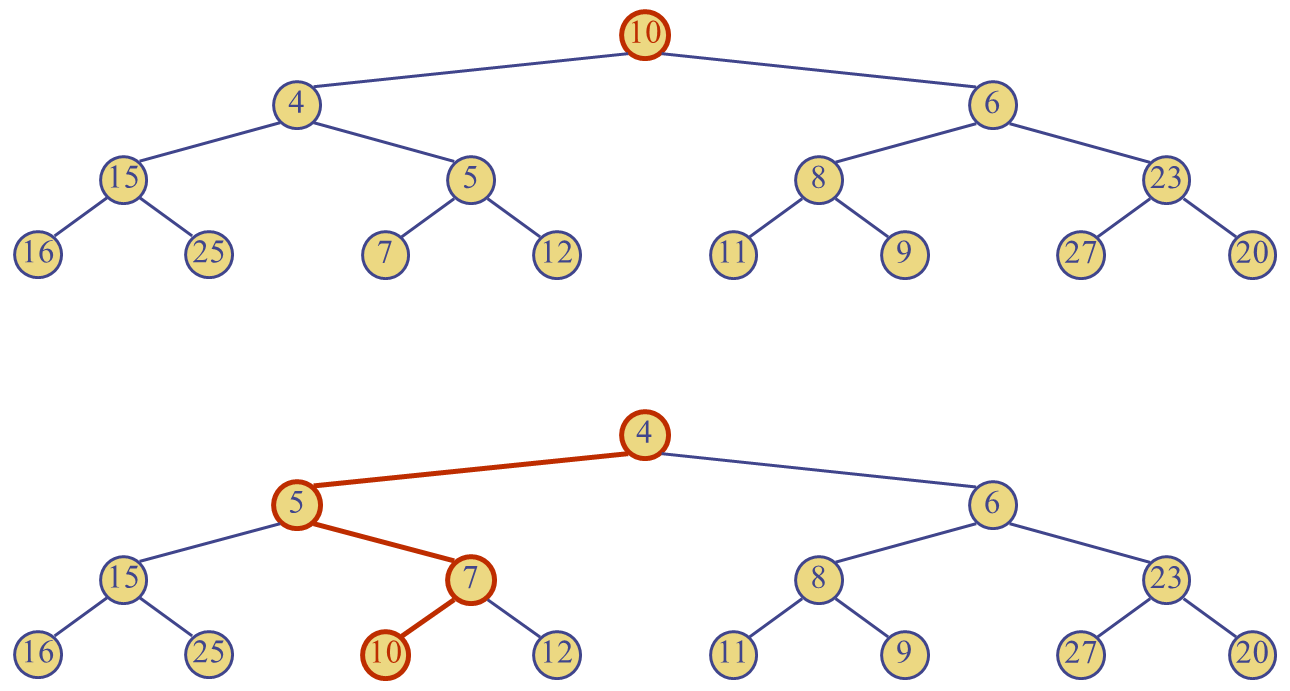
\includegraphics[width=10cm]{asp-09-pic17.png}
  \end{center}
\end{frame}

\begin{frame}[fragile]
  \frametitle{Analiza konstrukcije heapa}
  \begin{itemize}
    \item najgori slučaj za downheap: prvo krene desno pa onda stalno levo do
    dna heapa
    \item svaki čvor se obiđe u najviše dve putanje
    \item ukupan broj čvorova u putanjama je $O(n)$
    \item bottom-up konstrukcija heapa radi u $O(n)$ vremenu
    \item bottom-up konstrukcija heapa je brža nego $n$ dodavanja u heap sa upheap korekcijom
  \end{itemize}
  \begin{center}
    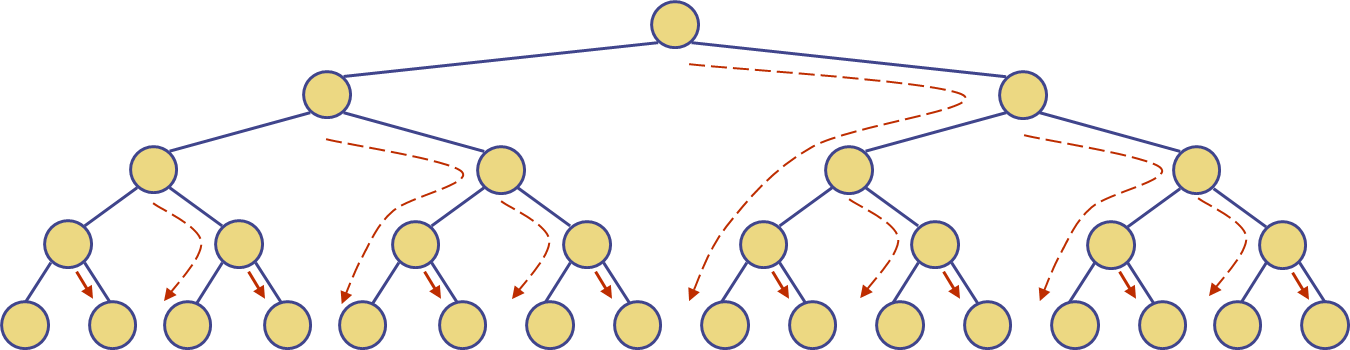
\includegraphics[width=10cm]{asp-09-pic18.png}
  \end{center}
\end{frame}

\section[Adaptivni RSP]{Adaptivni red sa prioritetom}
\begin{frame}[fragile]
  \frametitle{Adaptivni red sa prioritetom}
  \begin{itemize}
    \item \textbf{primer}: sistem za kupoprodaju akcija koristi dva reda sa
    prioritetom, jedan za prodaju i drugi za kupovinu sa elementima ($p, s$)
    \begin{itemize}
      \item ključ $p$ je cena
      \item vrednost $s$ je broj akcija
      \item nalog za kupovinu ($p, s$) se izvršava kada se pojavi nalog za
      prodaju ($p', s'$) sa cenom $p'\leq p$ (postupak je završen ako $s'\geq
      s$)
      \item nalog za prodaju ($p, s$) se izvršava kada se pojavi nalog za
      kupovinu ($p', s'$) sa cenom $p'\leq p$ (postupak je završen ako $s'\geq
      s$)
    \end{itemize}
    \item šta ako neko hoće da otkaže nalog pre nego što se izvrši?
    \item šta ako neko hoće da izmeni cenu ili broj akcija?
  \end{itemize}
\end{frame}

\begin{frame}[fragile]
  \frametitle{Adaptivni red sa prioritetom: operacije}
  \begin{itemize}
    \item \myred{remove}(loc): ukloni i vrati element $e$ iz reda za lokator
    $loc$
    \item \myred{update}(loc, k, v): zameni ključ/vrednost par ($k, v$) za
    lokator $loc$
  \end{itemize}
\end{frame}

\begin{frame}[fragile]
  \frametitle{Lokatori}
  \begin{itemize}
    \item element sa lokatorom identifikuje i prati poziciju ($k, v$) unutar
    strukture podataka
    \item primeri:
    \begin{itemize}
      \item broj kaputa u garderobi
      \item broj rezervacije 
    \end{itemize}
    \item osnovna ideja:
    \begin{itemize}
      \item pošto elemente kreira i vraća sama struktura podataka, oni mogu biti
      takvi da pamte svoju lokaciju, što pojednostavljuje kasnije ažuriranje
    \end{itemize}
  \end{itemize}
\end{frame}

\begin{frame}[fragile]
  \frametitle{Lokatori i liste}
  \begin{itemize}
    \item element liste čuva
    \begin{itemize}
      \item ključ
      \item vrednost
      \item poziciju 
    \end{itemize}
    \item reference se ažuriraju u \textbf{swap} operaciji
  \end{itemize}
  \begin{center}
    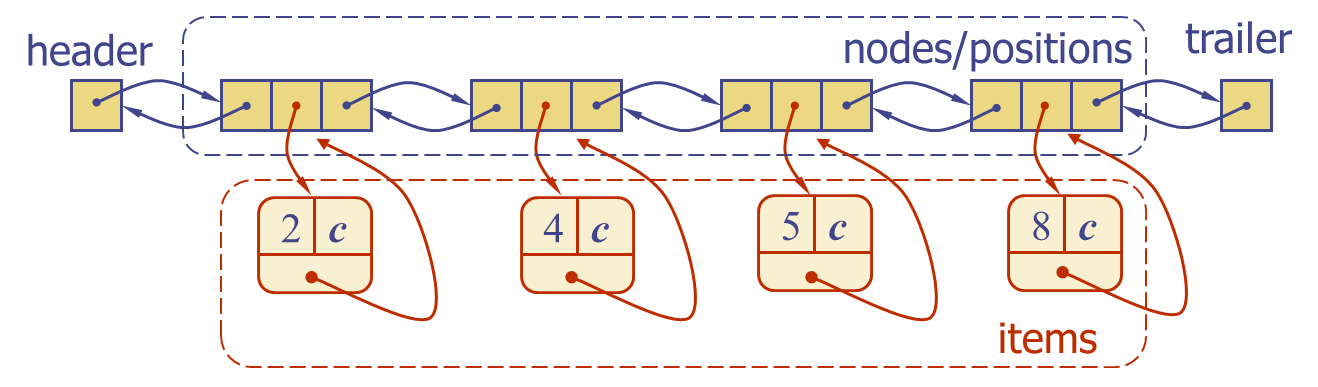
\includegraphics[width=10cm]{asp-09-pic19.png}
  \end{center}
\end{frame}

\begin{frame}[fragile]
  \frametitle{Lokatori i heap}
  \begin{columns}
    \begin{column}[c]{5cm}
      \begin{itemize}
        \item element heapa čuva
        \begin{itemize}
          \item ključ
          \item vrednost
          \item poziciju 
        \end{itemize}
        \item reference se ažuriraju u \textbf{swap} operaciji
      \end{itemize}
    \end{column}
    \begin{column}[c]{6cm}
      \begin{center}
        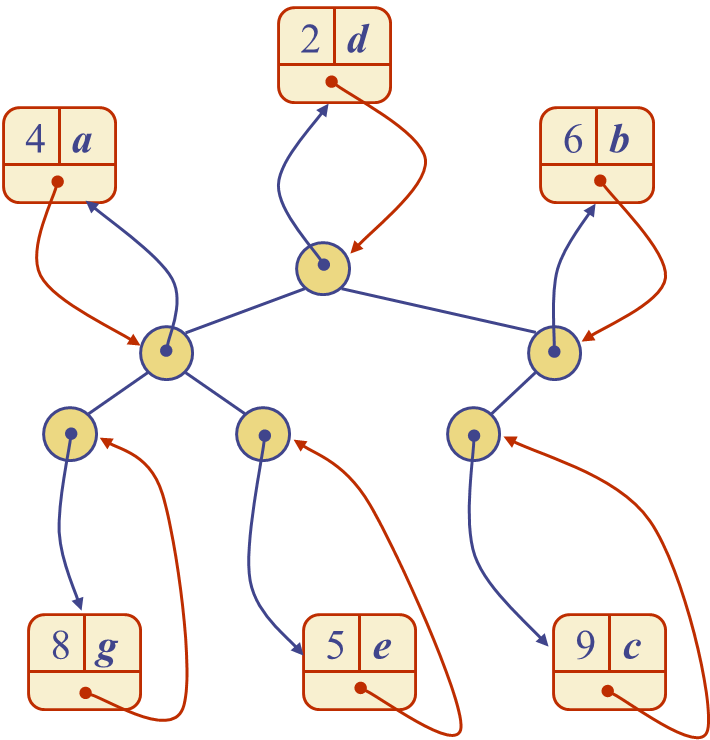
\includegraphics[width=6cm]{asp-09-pic20.png}
      \end{center}
    \end{column}
  \end{columns}
\end{frame}

\begin{frame}[fragile]
  \frametitle{Performanse}
  \begin{itemize}
    \item dobici u brzini usled korišćenja lokatora su označeni \myred{crveno} 
  \end{itemize}
  \begin{center}
    \begin{tabular}{llll}
      \textbf{metoda} & \textbf{nesortirana lista} & \textbf{sortirana lista} & \textbf{heap} \\ \hline\hline
      \texttt{len}, \texttt{is\_empty} & $O(1)$ & $O(1)$ & $O(1)$ \\ \hline
      \texttt{add} & $O(1)$ & $O(n)$ & $O(\log n)$ \\ \hline
      \texttt{min} & $O(n)$ & $O(1)$ & $O(1)$ \\ \hline
      \texttt{remove\_min} & $O(n)$ & $O(1)$ & $O(\log n)$ \\ \hline
      \texttt{remove} & \myred{$O(1)$} & \myred{$O(1)$} & \myred{$O(\log n)$} \\ \hline
      \texttt{update} & \myred{$O(1)$} & $O(n)$ & \myred{$O(\log n)$} \\ \hline
    \end{tabular}
  \end{center}
\end{frame}

\section[Sortiranje]{Strukture podataka i sortiranje}
\begin{frame}[fragile]
  \frametitle{Red sa prioritetom i sortiranje}
  \begin{columns}
    \begin{column}[c]{5cm}
      \begin{itemize}
        \item možemo upotrebiti red sa prioritetom za sortiranje niza elemenata
        \begin{itemize}
          \item dodamo elemente jedan po jedan putem \myred{add} operacije
          \item uklonimo elemente jedan po jedan putem \myred{remove\_min} operacije
        \end{itemize}
        \item vreme izvršavanja zavisi od načina implementacije
      \end{itemize}
    \end{column}
    \begin{column}[c]{6cm}
    \myred{PQ\_sort}($S, C$)
    \begin{algorithmic}
      \REQUIRE sekvenca $S$, komparator $C$
      \ENSURE rastuće sortirana $S$ u skladu sa $C$
      \STATE $P \leftarrow$ RSP sa komparatorom $C$
      \WHILE{$\neg S$.is\_empty()}
        \STATE $e\leftarrow S$.remove\_first()
        \STATE $P$.add($e, \emptyset$)
      \ENDWHILE
      \WHILE{$\neg P$.is\_empty()}
        \STATE $e \leftarrow P$.remove\_min().key()
        \STATE $S$.add\_last($e$)
      \ENDWHILE
    \end{algorithmic}    
    \end{column}
  \end{columns}
\end{frame}

\begin{frame}[fragile]
  \frametitle{Selection sort}
  \begin{itemize}
    \item \myred{selection sort} je varijanta PQ-sorta gde je RSP implementiran pomoću \textbf{nesortirane} liste
    \item vreme izvršavanja selection sorta:
    \begin{itemize}
      \item dodavanje $n$ elemenata u RSP traje $O(n)$
      \item uklanjanje $n$ elemenata u sortiranom redosledu traje \\
      $$1 + 2 + \ldots + n$$ 
    \end{itemize}
    \item selection sort radi u $O(n^2)$ vremenu
  \end{itemize}
\end{frame}

\begin{frame}[fragile,shrink]
  \frametitle{Selection sort: primer}
  \begin{center}
    \begin{tabular}{lll}
       & \textbf{sekvenca $S$} & \textbf{red $P$} \\ \hline\hline
      \textit{ulaz:} & $(7,4,8,2,5,3,9)$ & $()$ \\ \hline
      \textit{faza 1} &  & \\ 
      (a) & $(4,8,2,5,3,9)$ & $(7)$ \\ 
      (b) & $(8,2,5,3,9)$ & $(7,4)$ \\ 
      \ldots & \ldots & \ldots \\
      (g) & $()$ & $(7,4,8,2,5,3,9)$ \\ \hline
      \textit{faza 2} &  & \\ 
      (a) & $(2)$ & $(7,4,8,5,3,9)$ \\ 
      (b) & $(2,3)$ & $(7,4,8,5,9)$ \\ 
      (c) & $(2,3,4)$ & $(7,8,5,9)$ \\ 
      (d) & $(2,3,4,5)$ & $(7,8,9)$ \\ 
      (e) & $(2,3,4,5,7)$ & $(8,9)$ \\ 
      (f) & $(2,3,4,5,7,8)$ & $(9)$ \\ 
      (g) & $(2,3,4,5,7,8,9)$ & $()$
    \end{tabular}
  \end{center}
\end{frame}

\begin{frame}[fragile]
  \frametitle{Insertion sort}
  \begin{itemize}
    \item \myred{insertion sort} je varijanta PQ-sorta gde je RSP implementiran pomoću \textbf{sortirane} liste
    \item vreme izvršavanja insertion sorta:
    \begin{itemize}
      \item dodavanje $n$ elemenata u RSP traje \\
      $$1 + 2 + \ldots + n$$ 
      \item uklanjanje $n$ elemenata traje $O(n)$
    \end{itemize}
    \item insertion sort radi u $O(n^2)$ vremenu
  \end{itemize}
\end{frame}

\begin{frame}[fragile,shrink]
  \frametitle{Insertion sort: primer}
  \begin{center}
    \begin{tabular}{lll}
       & \textbf{sekvenca $S$} & \textbf{red $P$} \\ \hline\hline
      \textit{ulaz:} & $(7,4,8,2,5,3,9)$ & $()$ \\ \hline
      \textit{faza 1} &  &   \\ 
      (a) & $(4,8,2,5,3,9)$ & $(7)$ \\ 
      (b) & $(8,2,5,3,9)$ & $(4,7)$ \\ 
      (c) & $(2,5,3,9)$ & $(4,7,8)$ \\ 
      (d) & $(5,3,9)$ & $(2,4,7,8)$ \\ 
      (e) & $(3,9)$ & $(2,4,5,7,8)$ \\ 
      (f) & $(9)$ & $(2,3,4,5,7,8)$ \\ 
      (g) & $()$ & $(2,3,4,5,7,8,9)$ \\ \hline 
      \textit{faza 2} &  &   \\ 
      (a) & $(2)$ & $(3,4,5,7,8,9)$ \\
      (b) & $(2,3)$ & $(4,5,7,8,9)$ \\
      \ldots & \ldots & \ldots \\ 
      (g) & $(2,3,4,5,7,8,9)$ & $()$
    \end{tabular}
  \end{center}
\end{frame}

\begin{frame}[fragile]
  \frametitle{Sortiranje unutar iste strukture podataka (in-place)}
  \begin{columns}
    \begin{column}[c]{6cm}
      \begin{itemize}
        \item umesto korišćenja 2 strukture možemo implementirati selection i insertion sort u okviru jedne strukture
        \item deo ulaznog niza će poslužiti kao RSP
        \item za insertion sort
        \begin{itemize}
          \item držimo sortiran početak niza
          \item elemente menjamo pomoću \myred{swap} operacije
        \end{itemize}
      \end{itemize}
    \end{column}
    \begin{column}[c]{5cm}
      \begin{center}
        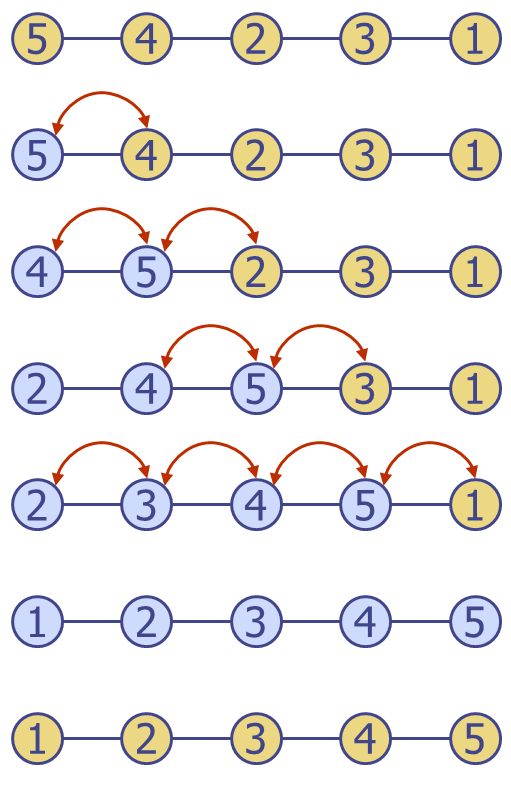
\includegraphics[width=4.5cm]{asp-09-pic21.png}
      \end{center}
    \end{column}
  \end{columns}
\end{frame}

\begin{frame}[fragile]
  \frametitle{Heap sort}
  \begin{columns}
    \begin{column}[c]{6cm}
      \begin{itemize}
        \item posmatramo RSP sa $n$ elemenata, implementiran pomoću heapa
        \begin{itemize}
          \item potreban prostor je $O(n)$
          \item \myred{add} i \myred{remove\_min} traju $O(\log n)$
          \item \myred{len}, \myred{is\_empty}, \myred{min} traju $O(1)$
        \end{itemize}
      \end{itemize}
    \end{column}
    \begin{column}[c]{6cm}
      \begin{itemize}
        \item ovakav RSP možemo koristiti za sortiranje $n$ elemenata za $O(n\log n)$ vreme
        \item rezultujući algoritam se zove \myred{heap sort}
        \item znatno brži od kvadratnih algoritama kao što su selection i insertion sort
      \end{itemize}
    \end{column}
  \end{columns}
  $$O(n\log n) < O(n^2)$$
\end{frame}

\end{document}
